\documentclass{beamer}
%\documentclass[handout]{beamer}
\usetheme{Malmoe}
\bibliographystyle{turabian}

\setbeamertemplate{navigation symbols}{}%remove navigation symbols
\setbeamertemplate{bibliography item}[triangle] %don't use icons in references

\setbeamertemplate{headline}{%
\leavevmode%
  \hbox{%
    \begin{beamercolorbox}[wd=\paperwidth,ht=2.5ex,dp=1.125ex]{palette quaternary}%
    \insertsectionnavigationhorizontal{\paperwidth}{\hskip0pt plus1filll}{\hskip0pt plus1filll}
    \end{beamercolorbox}%
  }
}

\usepackage{fancyhdr}
\usepackage{graphicx}
\usepackage{subfigure}
\usepackage{listings}
\usepackage{mathtools}
\setbeamertemplate{itemize items}[circle]
\setbeamertemplate{caption}[numbered]

\title[Dithered Index]{Dithered Index}
\subtitle{An Experiment in Dithering and Texture Compression}
\author{Diana Arrieta}
\date{\today}

\begin{document}

\begin{frame}
\titlepage
\end{frame}

\section[]{Outline}
\begin{frame}
  \tableofcontents
\end{frame}

\section{Introduction}
\begin{frame}
   \frametitle{Introduction}
   Texture Compression
   \begin{itemize}
   \item{Intro}
      \begin{itemize}
      \item{What is it?}
      \end{itemize}
   \pause
   \item{Motivation}
   \pause
      \begin{itemize}
      \item{Smaller: Decreased Storage Requirements}
   \pause
      \item{Faster: Decreased Bandwidth Requirements}
   \pause
      \item{Better: More Information Can Be Stored}
   \pause
      \end{itemize}
   \item{Applications}
   \pause
      \begin{itemize}
      \item{Video Games}
      \item{Simulations}
      \item{Rendering}
      \item{Medical Settings, etc.}
      \end{itemize}
   \end{itemize}
\end{frame}

\section{Human Vision}
\begin{frame}
   \frametitle{Human Vision}
   The human eye...
   \begin{figure}[!htbp]
   \begin{center}
   \subfigure{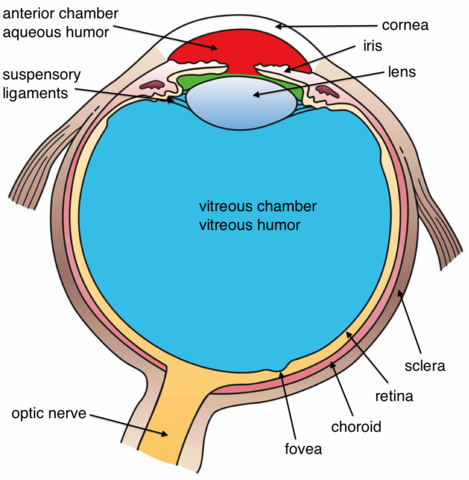
\includegraphics[scale=.5]{./images/diagrams/eye_structures}}
   \end{center}
   \end{figure}
   
   \begin{itemize}
   \item{Can perceive about 10 million colors}
   \begin{itemize}
      \item{Compare that to 16.7 million colors on your 24-bit LCD screen!}
   \end{itemize}
   \end{itemize}
\end{frame}

\begin{frame}
   A visual exploit...
   \begin{itemize}
   \item{Difficult to differentiate between similar colors.}
   \end{itemize}
\end{frame}

\begin{frame}
   \begin{figure}[!htbp]
   \begin{center}
   \subfigure{
\includegraphics[scale=0.5]{./images/diagrams/red147}}
   \end{center}
   \end{figure}
\end{frame}

\begin{frame}
   A different visual exploit...
   \begin{itemize}
   \item{Perceived colors are subject to lighting conditions and context.}
   \end{itemize}
\end{frame}

\begin{frame}
   \begin{figure}[!htbp]
   \begin{center}
   \subfigure{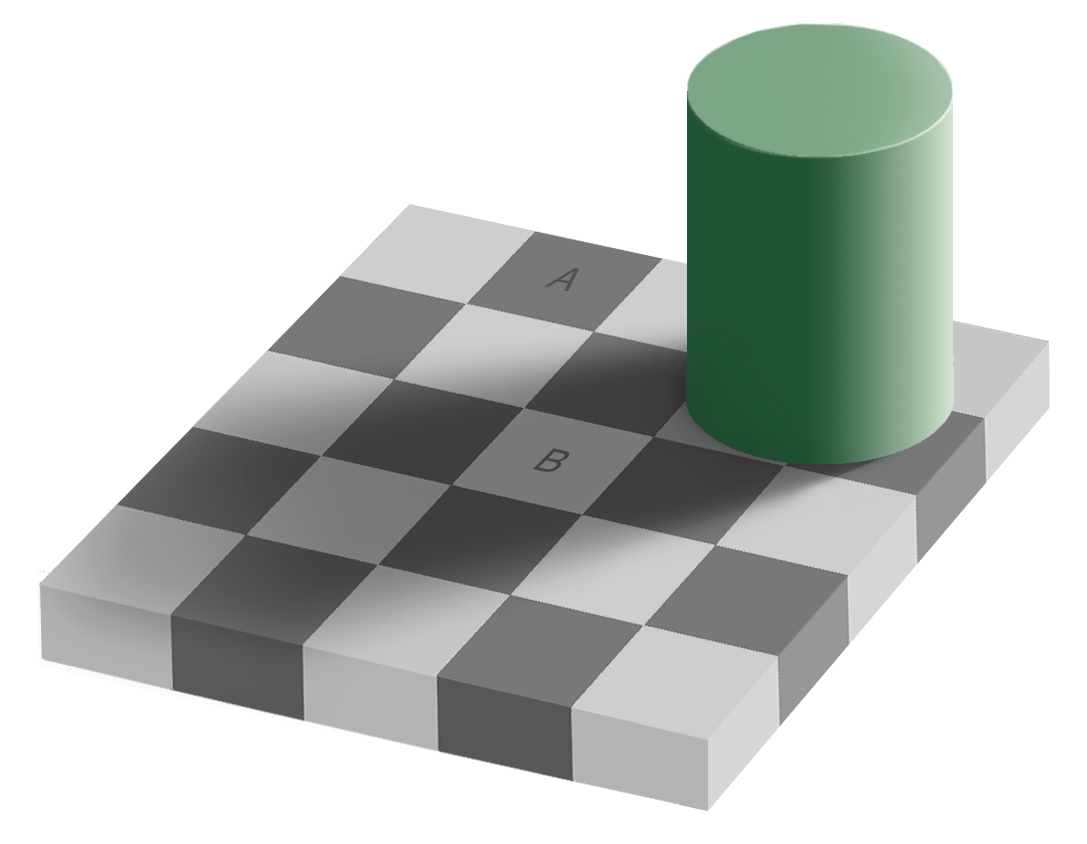
\includegraphics[scale=0.2]{./images/diagrams/grey_square}}
   \end{center}
   \end{figure}
\end{frame}

\begin{frame}
   \begin{figure}[!htbp]
   \begin{center}
   \subfigure{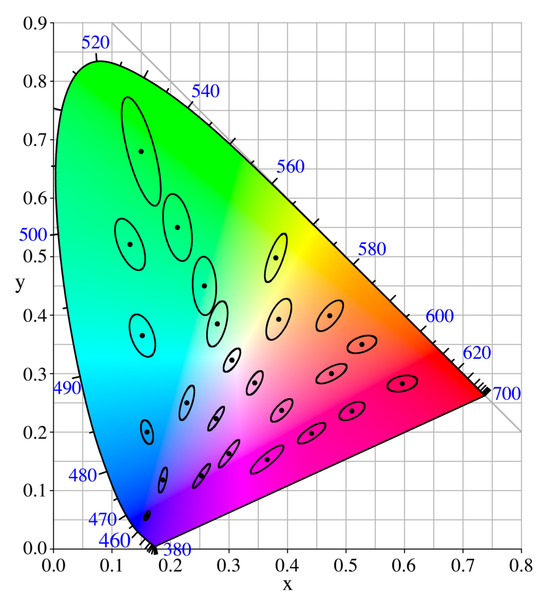
\includegraphics[scale=0.30]{./images/diagrams/macadam}}
   \caption{MacAdam ellipses shown ten times their actual size on the CIE 1931 XYZ color space. Colors inside an ellipse visually match the color in the center.}
   \end{center}
   \end{figure}
\end{frame}

\section{Dithering}

\begin{frame}
   \frametitle{Dithering}
   \begin{itemize}
   \item{An optical illusion of color depth in where colors not available in the provided palette are approximated by placing similar colors in a pattern to achieve the desired color.}
   \end{itemize}
\end{frame}

\begin{frame}
   \begin{figure}[!hbp]
   \begin{center}
   \subfigure{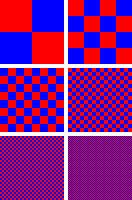
\includegraphics[scale=1]{./images/compress/dithering}}
   \subfigure{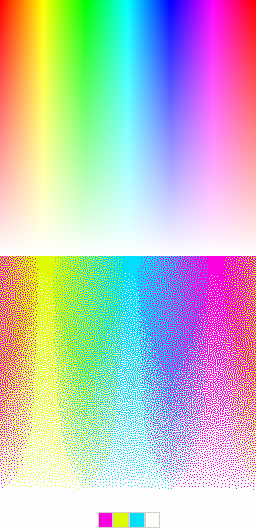
\includegraphics[scale=0.38]{./images/compress/rainbow_dithering}}
   \caption{Using dithering, more colors can be represented using a reduced color palette.}
   \end{center}
   \end{figure}   
\end{frame}

\begin{frame}
   \begin{figure}[!htbp]
   \begin{center}
   \subfigure{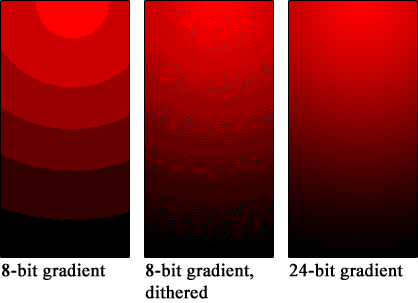
\includegraphics[scale=0.6]{./images/compress/banding_gradient}}
   \caption{Banding in a gradient. Banding is reduced when dithering is applied.}
   \end{center}
   \end{figure}   
\end{frame}

\begin{frame}
   \begin{itemize}
   \item{What's the difference between Dithering and Half-toning?}
   \pause
      \begin{itemize}
      \item{Half-toning uses CMYK colors, varying dot sizes, and overlapping techniques to achieve the color desired.}
      \end{itemize}
   \end{itemize}
   
   \pause
   \begin{figure}[!htbp]
   \begin{center}
   \subfigure{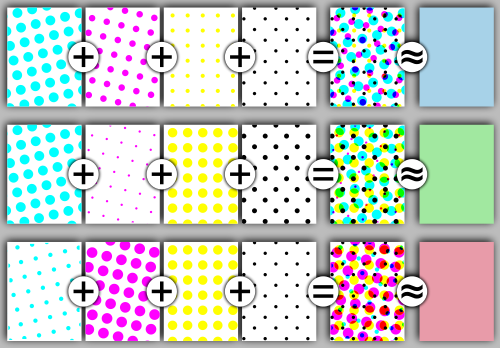
\includegraphics[scale=0.5]{./images/diagrams/halftoning}}
   \end{center}
   \end{figure}
   
\end{frame}

\section{Compression}
\begin{frame}
   \frametitle{Compression}
   Involves encoding information into fewer bits than would otherwise be occupied by the original source.
\end{frame}

\begin{frame}
   \frametitle{Lossless Compression Methods}
   Definition: A data encoding method that removes redundancies and uses fewer bits to represent the same data. (Best uses: Text or Archiving.)
\end{frame}

\begin{frame}
   \frametitle{Huffman Encoding}
   \begin{itemize}
   \item{An entropy encoder that substitutes more common characters with fewer bits, while infrequent characters are encoded with more bits.}
   \pause
   \item{Average Compression: 2.3 to 2.9 bits per character (8 bits)}
   \item{Cons: Requires two passes to build variable length codes.}
      \begin{itemize}
      \item{You can use pre-built trees to encode rather than building one.}
      \end{itemize}
   \end{itemize}
\end{frame}

\begin{frame}
\begin{center}
\begin{figure}[!htbp]
\begin{tabular}{| l | l | l | l | l | l | l | l |}
\hline
Letter & Frequency & Letter & Frequency\\ \hline
e & 0.12702 & w & 0.02360 \\ \hline
t & 0.09056 & f & 0.02228 \\ \hline
a & 0.08167 & g & 0.02015 \\ \hline
o & 0.07507 & y & 0.01974 \\ \hline
i & 0.06966 & p & 0.01929 \\ \hline
n & 0.06749 & b & 0.01492 \\ \hline
s & 0.06327 & v & 0.00978 \\ \hline
h & 0.06094 & k & 0.00772 \\ \hline
r & 0.05987 & j & 0.00153 \\ \hline
d & 0.04253 & x & 0.00150 \\ \hline
l & 0.04025 & q & 0.00095 \\ \hline
c & 0.02782 & z & 0.00074 \\ \hline
u & 0.02758 &   &         \\ \hline
m & 0.02406 &   &         \\ \hline
\end{tabular}
\caption{Frequency for common letters in the English language.}
\end{figure}
\end{center}
\end{frame}

\begin{frame}
\begin{figure}[!htbp]
\begin{center}
\subfigure{\includegraphics[scale=1]{./images/diagrams/Morse}}
\caption{A Huffman binary tree. This is the tree also used for Morse code.}
\end{center}
\end{figure}
\end{frame}

\begin{frame}
   \frametitle{Lempel-Ziv-Welch}
   \begin{itemize}
   \item{ As the algorithm encounters patterns that it has seen before, it substitutes these with a shorter representation provided that it is already in the dictionary. If not, it creates one on the spot and outputs the corresponding code.}
   \pause
   \item{Average Compression: 2 bits per character (8 bits)}
   \pause
   \item{Different files construct different dictionaries which do not need to be stored.}
   \pause
   \item{Can create substitutions for entire strings rather than single characters.}
   \pause
   \item{In longer files, a better compression ratio can often be achieved since a large dictionary has a better chance of finding matches.}
   \pause
   \item{Tradeoff: A large dictionary can find more matches at the cost of processing time.}
   \end{itemize}
\end{frame}

\begin{frame}[fragile]
\begin{quote}
\begin{figure}[!htbp]
\begin{verbatim}
w = NIL;
   while ( read a character k )
   {
      if wk exists in the dictionary
         w = wk;
      else
         add wk to the dictionary;
      output the code for w;
      w = k;
   }
\end{verbatim}
\caption{Pseudo-code for LZW (compression).}
\end{figure}
\end{quote}
\end{frame}

\begin{frame}[fragile]
\begin{figure}[!htbp]
\begin{verbatim}
read a character k;
   output k;
   w = k;
   while ( read a character k )
   /* k could be a character or a code. */
   {
      if k exists in the dictionary
         entry = dictionary entry for k;
         output entry;
         add w + entry[0] to dictionary;
         w = entry;
      else
         output entry = w + firstCharacterOf(w);
      add entry to dictionary;
      w = entry;
   }
\end{verbatim}
\caption{Pseudo-code for LZW (decompression).}
\end{figure}
\end{frame}


\begin{frame}
   \frametitle{Lossy Compression Methods}
   Definition: A data encoding method that discards some data in order to achieve compression. The resulting data is similar enough to the original data. (Best uses: Images, Audio, Video.)
\end{frame}

\begin{frame}
   \frametitle{Lossy: Wavelet Transform}
   \begin{itemize}
   \item{Becomes lossy when coefficients that don't meet the threshold are reduced to zero.}
   \item{Is first performed over rows, then columns.}
   \item{Most of the resulting data is discarded, with high level data in the upper left, and smaller details to the lower right.}
   \end{itemize}
\end{frame}


\begin{frame}[fragile]
   \frametitle{Lossy: Wavelet Transform}
   \begin{verbatim}
   7   1   6   6   3   -5   4   2

   Averages:
   (7 +  1) / 2 =  4
   (6 +  6) / 2 =  6
   (3 + -5) / 2 = -1
   (4 +  2) / 2 =  3

   Differences:
   (7 -  4) = ( 4 -  1) = 3
   (6 -  6) = ( 6 -  6) = 0
   (3 - -1) = (-1 - -5) = 4
   (4 -  3) = ( 3 -  2) = 1

   Resulting array:
   4   6   -1   3	  3   0   4   1

   \end{verbatim}
\end{frame}

\begin{frame}
   \frametitle{Lossy: Wavelet Transform}
   \pause
   \begin{figure}[!htbp]
   \begin{center}
   \subfigure{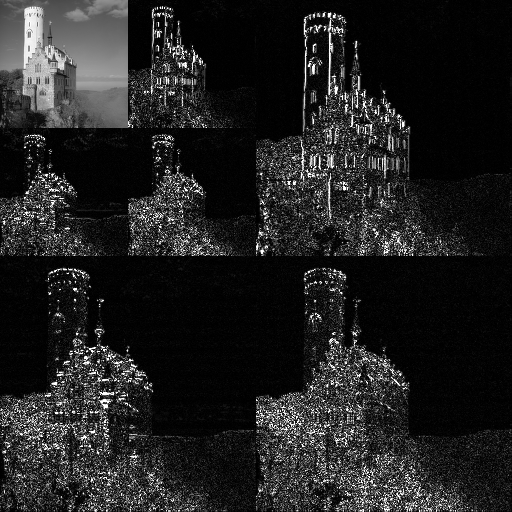
\includegraphics[scale=0.25]{./images/compress/wavelet}}
   \subfigure{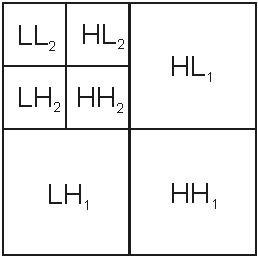
\includegraphics[scale=.5]{./images/compress/dia_wavelet}}
   \caption{Image processed with a wavelet transform. Each block contains coefficients to reconstruct the original image.}
   \end{center}
   \end{figure}
\end{frame}

   
\begin{frame}
   \frametitle{Lossy: Motion Compensation}
   Compensates for differences between subsequent frames.
   \begin{itemize}
   \item{MPEG-2}
      \begin{itemize}
      \item{I-Frame: Initial Frame.}
      \pause
      \item{P-Frame: Predicted Frame or Delta Frame. Holds changes that occur between frames. Holds less data than a full frame.}
      \pause
      \item{B-Frame: Bi-directional frame. Contains forward and backward prediction of the closest I-Frame and P-frame.}
      \end{itemize}
   \end{itemize}
\end{frame}

\begin{frame}
   \begin{center}
   \begin{figure}[!htbp]
   \subfigure{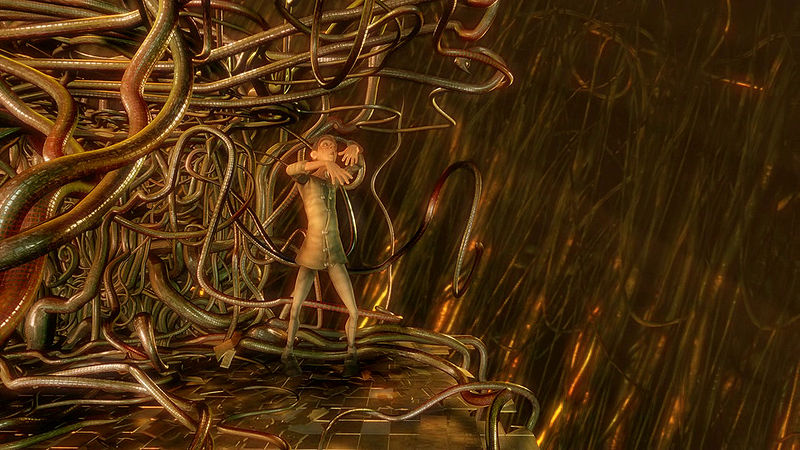
\includegraphics[scale=0.18]{./images/compress/original}}
   \subfigure{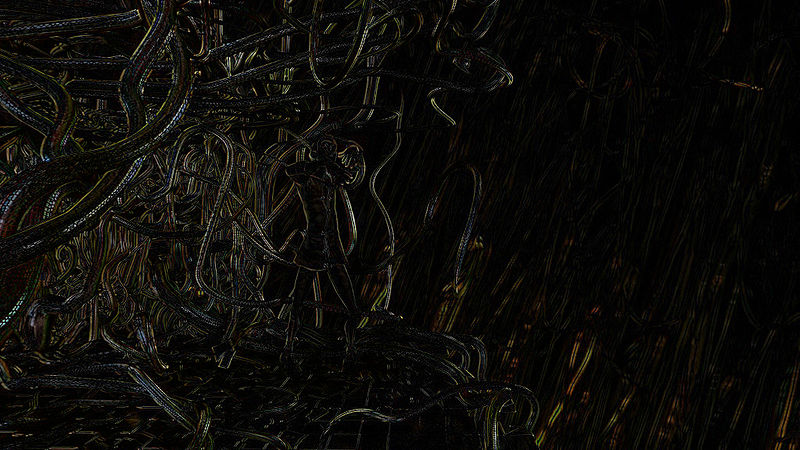
\includegraphics[scale=0.18]{./images/compress/difference}}
   \subfigure{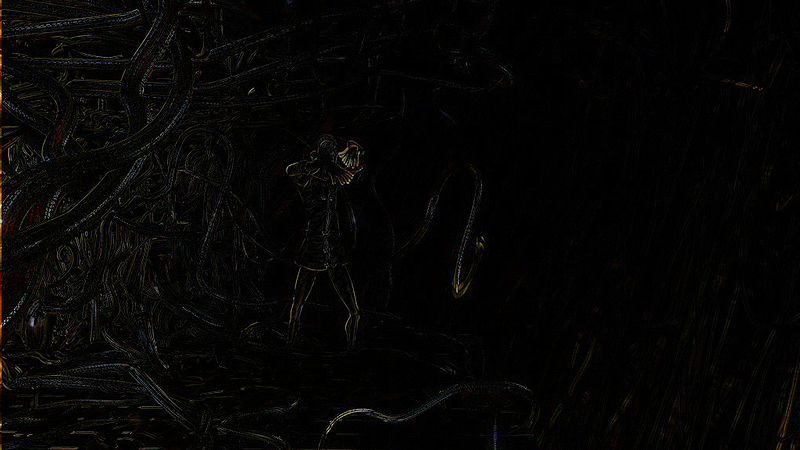
\includegraphics[scale=0.18]{./images/compress/motion}}
   \caption{The original frame, the difference frame, and the motion compensated frame.}
   \end{figure}
   \end{center}
\end{frame}

\section{Textures}
\begin{frame}
   \frametitle{Textures}
   Images that are intended to be mapped to a surface. They are highly compressed using fixed-rate compression algorithms, and are also quick to decompress, either as a whole or just a section.
   
   \begin{itemize}
   \item{Can contain:}
      \begin{itemize}
     \pause
      \item{Terrain, usually grass, concrete, etc. (Typically flat)}
      \item{Object surfaces, such as boxes, furniture, etc. (Can be irregular)}
      \item{Lighting information, dictating how light interacts with an object.}
      \end{itemize}
   \end{itemize}
\end{frame}

\begin{frame}
   \frametitle{Texture Atlas}
   Textures atlases contain a group of images...
   \pause
   \begin{figure}[!htbp]
   \begin{center}
   \subfigure{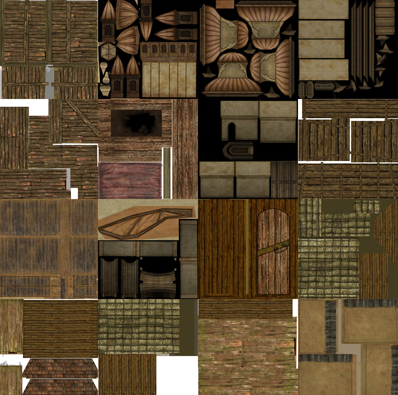
\includegraphics[scale=0.6]{./images/textures/texture_atlas}}
   \end{center}
   \end{figure}
\end{frame}

\begin{frame}
   \frametitle{Texture Synthesis}
   While synthesised textures are a single image that has been stitched to itself repeatedly to a larger resolution.
   \pause
   \begin{figure}[!htbp]
   \begin{center}
   \subfigure{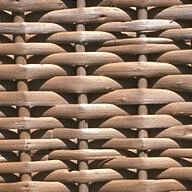
\includegraphics[scale=0.4]{./images/textures/basket}}
   \subfigure{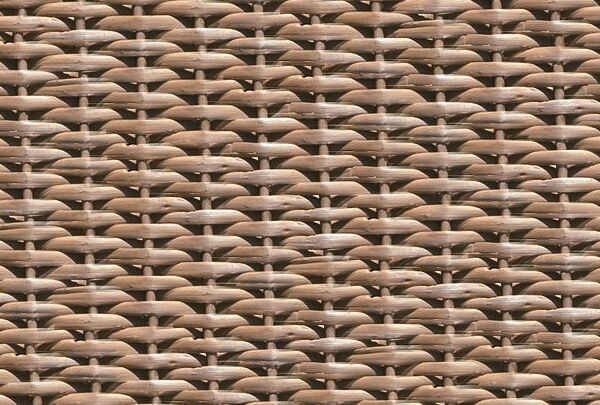
\includegraphics[scale=0.19]{./images/textures/basket_syn}}\\
   \subfigure{
\includegraphics[scale=0.7]{./images/textures/water}}
   \subfigure{
\includegraphics[scale=0.18]{./images/textures/water_syn}}
   \end{center}
\end{figure}
\end{frame}

\section{Texture Compression}
\begin{frame}
   \frametitle{Texture Compression}
   \begin{itemize}
   \item{Has Constraints:}
   \pause
      \begin{itemize}
      \item{Compressed ratio must be 1 to 4 or higher.}
      \pause
      \item{Decompression time must be lower than compression time.}
      \pause
      \item{Allow Random Access to individual blocks (fixed-rate compression).}
      \pause
      \item{Resulting decompressed images must look relatively similar.}
      \end{itemize}
   \end{itemize}
\end{frame}

\begin{frame}
   \frametitle{Current Standard: Direct X}
   \begin{itemize}
   \item{The current standard under Fixed-Rate Block Compression patent (S3TC).}
   \pause
      \begin{itemize}
      \item{Breaks images down to 4x4 blocks.}
      \pause
      \item{Finds a best fit line for a set of pixels.}
      \pause
      \item{Stores indexes of pixels along the line.}
      \pause
      \end{itemize}
   \item{Pros: Fast to decode and results in good compression.}
   \item{Con: If a value doesn't have a good fit to the line, it will not be represented accurately.}
   \end{itemize}
\end{frame}

\begin{frame}
   \begin{figure}[!htbp]
   \begin{center}
   \subfigure{\includegraphics[scale=0.7]{./images/textures/Shades_red}}\\
   \subfigure{
\includegraphics[scale=0.7]{./images/textures/Shades_colour}}
   \end{center}
   \caption{The errors for gradient textures is shown in the top set of images. The right shows the result of a reduced color palette, which cannot interpolate the original colors at all.}
   \end{figure}
\end{frame}

\begin{frame}
   \frametitle{Current Standard: Ericsson}
   Current standard used for Mobile Phones (notably Android)
   \begin{itemize}
   \item{Starts with a 4x4 block...}
      \begin{itemize}
      \item{Which is then broken down into a 4x2 or 2x4 block.}
      \item{Each part is given a singel base color (could be 4/4/4 or 5/5/5 RGB).}
      \item{Remaining bits are used to indicate the table used luminance values.}
      \end{itemize}
   \end{itemize}
\end{frame}

\begin{frame}
   \begin{figure}[!htbp]
   \begin{center}
   \subfigure{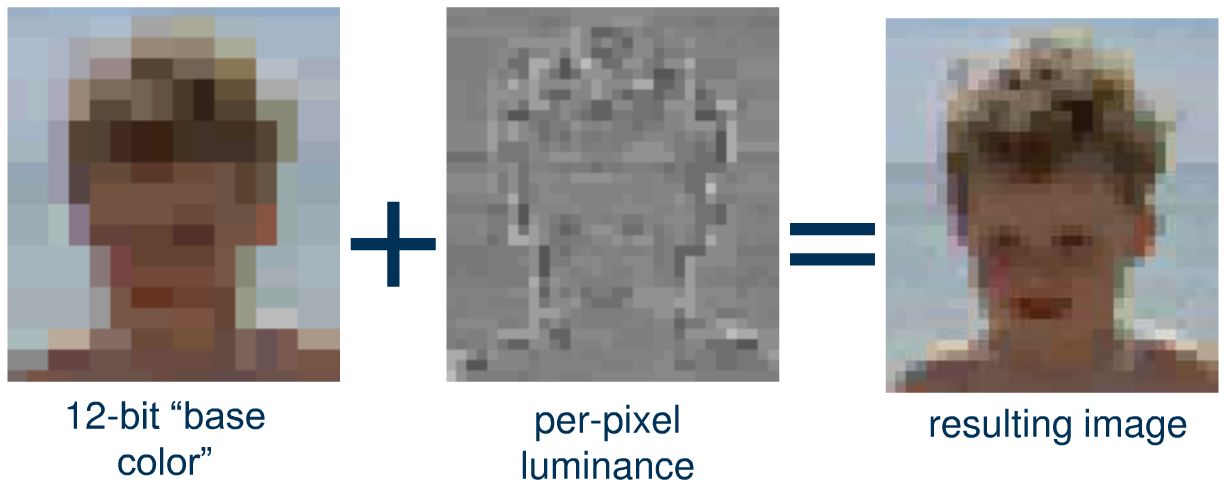
\includegraphics[scale=0.33]{./images/textures/ipackman}}
   \caption{The base colors are shown for each block on the left image, while luminance modulation is shown in the middle. The final image is the decompressed image.}
   \end{center}
   \end{figure}
\end{frame}

\section{Project Method}
\begin{frame}
   \frametitle{Project Method}
   \begin{itemize}
   \item{Relevance Dither}
   \item{Relevance Compression}
   \end{itemize}
\end{frame}

\begin{frame}[fragile]
   \frametitle{Relevance Dither}
\begin{verbatim}
      //Floyd-Steinberg
      //         X   7
      //     3   5   1
\end{verbatim}
\begin{verbatim}
      //Jarvis-Judice-Ninke
      //         X   7   5 
      // 3   5   7   5   3
      // 1   3   5   3   1
\end{verbatim}
\begin{verbatim}
      //Mine!
      //         X   4  1
      //         4   2
      //         1
\end{verbatim}

\end{frame}

\begin{frame}
   \frametitle{Relevance Compression}
   \begin{itemize}
   \item{Start with a 2x2 block.}
   \item{Convert pixel color to indexed color. (Keep count of this!)}
   \item{Find the most common indexes.}
   \item{Pixels that are not part of the most common indexes are changed to color that is part of this group.}
   \item{The best match is found using RGB as a distance coordinate, to find the next closest color.}
   \item{Save the most common indexes in the header.}
   \end{itemize}
\end{frame}

\section{Results}
\begin{frame}
   \frametitle{Results}
   \pause
   Pros:
   \begin{itemize}
   \item{Uses fewer colors.}
   \item{Smaller result than using Direct X.}
   \item{Compresses faster than Direct X.}
   \end{itemize}
   \pause
   Cons:
   \begin{itemize}
   \item{Does not outperform Direct X and Ericsson in decompression.}
   \item{The index sometimes does not include all the colors necessary to reconstruct the image at decompression time.}
   \end{itemize}
   \pause
   Suggestions:
   \begin{itemize}
   \item{Port to a language that doesn't use a virtual machine.}
   \item{Index tiles instead of single pixels.}
   \end{itemize}
\end{frame}

\section{Demo}
\begin{frame}
   \frametitle{Demo}
   \begin{figure}[!htbp]
   \begin{center}
   \subfigure{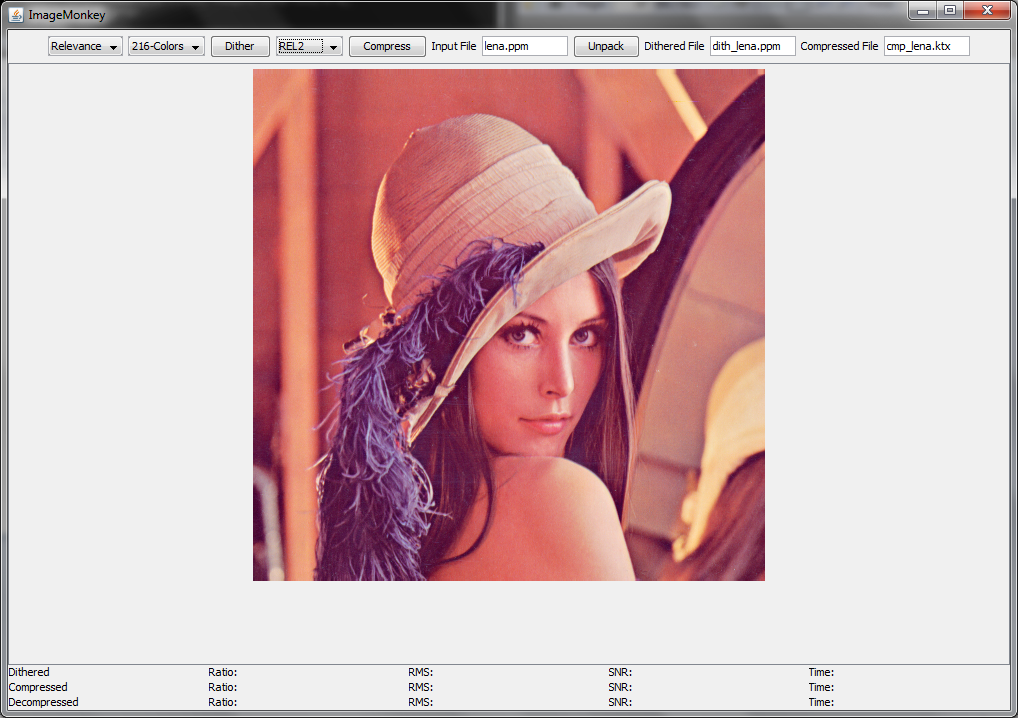
\includegraphics[scale=0.35]{./images/misc/java}}
   \end{center}
   \end{figure}
\end{frame}

\begin{frame}[allowframebreaks]
\def\newblock{\hskip .11em plus .33em minus .07em}
\frametitle{References}
\nocite{*}
\bibliography{bibfile}
\end{frame}

\end{document}
